\section{Data Quality} \label{sec:res_DataQuality}

%Initial hardware implementation show the accuracy of data from the eye tracker in question. A series of simple gaze fixation tests revealed the accuracy and noise inherent in the data produced, as well as the range of possible values full screen on a 24" 1920x1200 monitor. Data range was aquired by fixating on all four corners of the monitor. Accuracy and noise levels were measured in a steady, uninterrupted stream of gaze data where the user continually stared at a fixed point on screen for ten seconds. Test results are summarized in table \_.

Initial results presented will aim to paint a picture of the quality of data produced by the eye tracker detailed in section \ref{sec:hwds_TobiiEyeTracker5}. All results in this section were generated on a 24" 1920x1200 Dell monitor.

A general overview of data quality is presented in figure \ref{fig:res_GazePointTest}. This plot was generated by instructing the subject to fixate on nine different points for three seconds each. These nine points were chosen to observe how gaze is output at differing degrees of visual angle, as well as edge cases. The farthest points were at the four very edges of the monitor. One was at the center and the rest on the diagonals in between. Around 100 samples were collected for each gaze point. The test was subsequently repeated three times in a controlled environment. That is, with unchanged device calibration while disallowing the subject to move in the tracking space.

\begin{figure}[h]
    \centering
    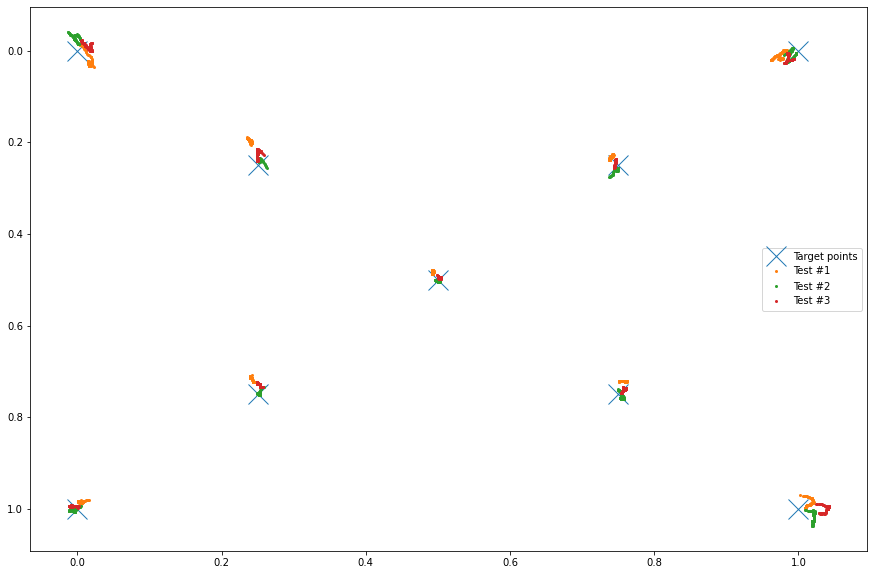
\includegraphics[width=\textwidth]{Images/DataQuality/GazePointTest.png}
    \caption{Gaze point test results. The x- and y-axes represent on-screen coordinates, as they are output from Tobii ET5. The blue crosses are the gaze points on which the user was instructed to fix their gaze. Orange, green, and red dots represent single-sample representations of user gaze in the first, second, and third tests, respectively.}
    \label{fig:res_GazePointTest}
\end{figure}

Next, the effects of data drift are given in figure \ref{fig:res_DataDeviations}. This plot is taken from the gaze point test of figure \ref{fig:res_GazePointTest} and is merely centered on and scaled up to only show the fine-grained evolution of gaze points during fixation. This particular point is at the top-left corner of the monitor. 

\begin{figure}[h]
    \centering
    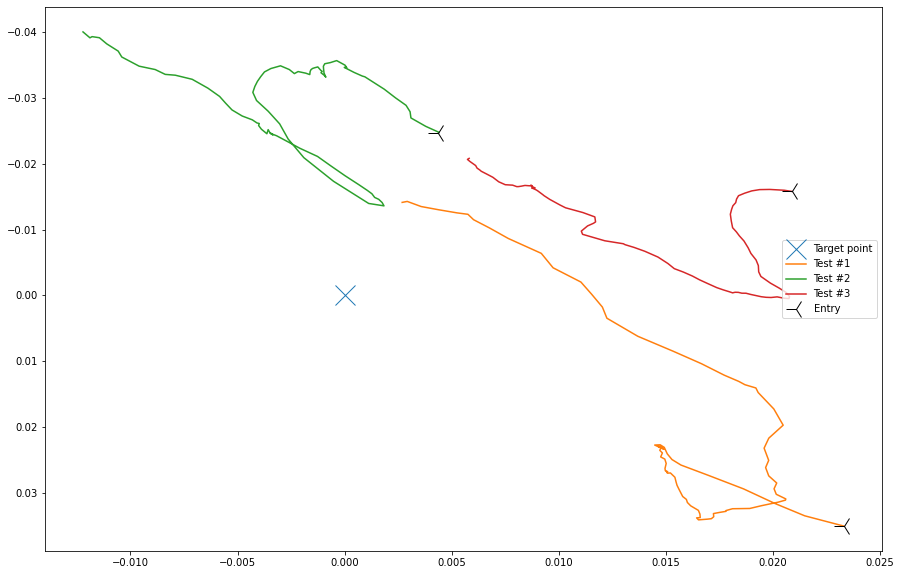
\includegraphics[width=\textwidth]{Images/DataQuality/DataDrift.png}
    \caption{Effects of data drift. Again, the x- and y-axes represent on-screen coordinates, as they are output from Tobii ET5. The single blue cross is the top-left target gaze point observable in figure \ref{fig:res_GazePointTest}. Orange, green, and red lines show the between-sample scan paths of user gaze in the first, second, and third tests, respectively. The black tri-crosses are the entry points from which the scan path evolves.}
    \label{fig:res_DataDrift}
\end{figure}

Another test was conducted to see whether scan paths produced by Tobii ET5 were consistent. This time, the subject was instructed to follow a moving target, traveling smoothly along all four borders of the monitor and along both diagonals. Again, the test was repeated three times. Each test lasted about 30 seconds, and around 3000 samples were collected in all.

\begin{figure}[h]
    \centering
    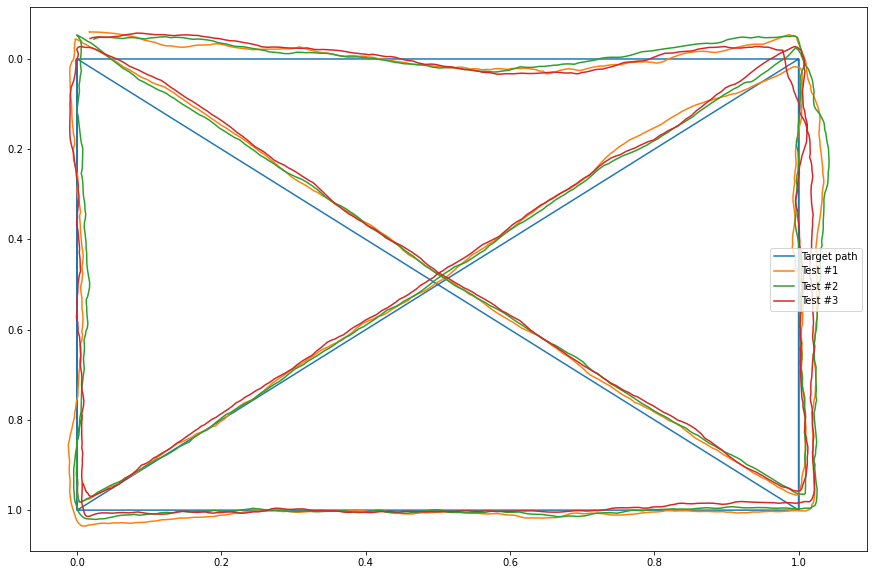
\includegraphics[width=\textwidth]{Images/DataQuality/ScanpathTest.png}
    \caption{Scan path test results. Once again, the x- and y-axes represent on-screen coordinates, as they are output from Tobii ET5. The straight blue lines are the target paths which the user was instructed to follow with their gaze. }
    \label{fig:res_ScanpathTest}
\end{figure}

Finally, to gain concrete insight into the fundamental statistical properties of the data stream, I present figure \ref{fig:res_DataDeviations}. These violin plots were all generated on the data gathered during the first gaze point test of figure \ref{fig:res_GazePointTest}. Each violin of each plot represent the deviations in on-screen coordinates of one point on one axis, from the mean of one observed set of data samples. Since the mean values of each point is subtracted from each violin, these plots do not account for bias. Each of these sets of data samples come from the user fixating at one of the nine gaze points of figure \ref{fig:res_GazePointTest}. Plots in the same column are generated from the same group of target gaze points, e.g. whether the point is at the screen edges, on the diagonal or in the center. The top row of plots show deviations in the y-coordinate axis, while the bottom row show the same on the x-axis.

\begin{figure}[h]
    \centering
    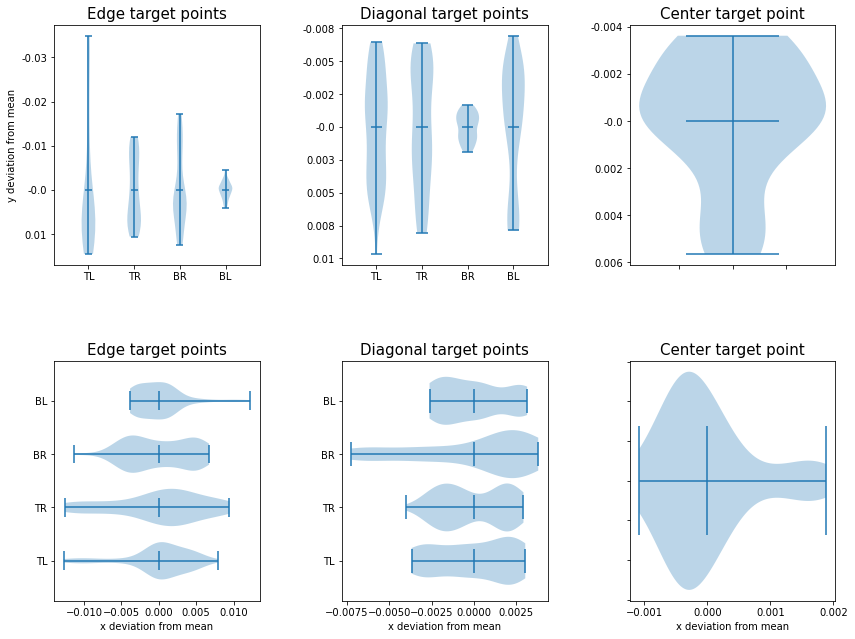
\includegraphics[width=\textwidth]{Images/DataQuality/DataDeviations.png}
    \caption{Data deviations. Columns share target gaze point types, rows share coordinate axes. For edge- and diagonal target plots, each violin represent either the top-left (TL), top-right (TR), bottom-right (BR), or bottom-left (BL) gaze target points. Note that the coordinate axes are scaled to match the values of each plot.}
    \label{fig:res_DataDeviations}
\end{figure}

Accompanying figure \ref{fig:res_DataDeviations} is table \ref{tab:res_DataStats}, which illustrates typical occurrences of bias and variance in the data output. As with figure \ref{fig:res_DataDeviations}, this data was gathered from the first gaze point test, representing related information. Additionally, bias is inferred by individually calculating the median position on both coordinate axes and subtracting the target point coordinates.

\import{./}{DataTable}

Figure \ref{fig:res_PaperHeatmap} attempts to illustrate data quality with a heat map. The left plot was generated by instructing the user to read one page of a paper, shown on the right. 
%As we can see, the eye tracker has an accuracy which allows for clear distinctions of paragraphs and lines.

\begin{figure}
    \centering
    \begin{minipage}{0.5\textwidth}
        \centering
        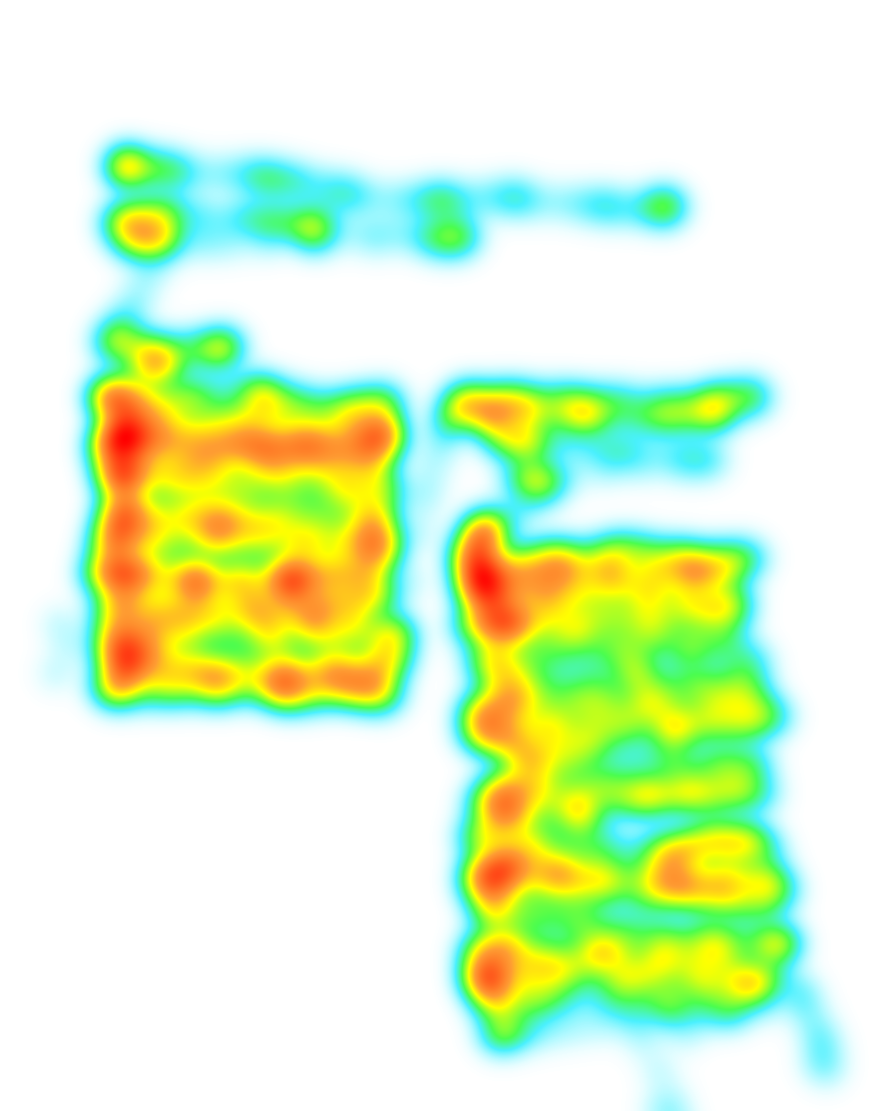
\includegraphics[width=\textwidth]{Images/DataQuality/PaperHeatmap.png}
        %\caption{first figure}
    \end{minipage}\hfill
    \begin{minipage}{0.5\textwidth}
        \centering
        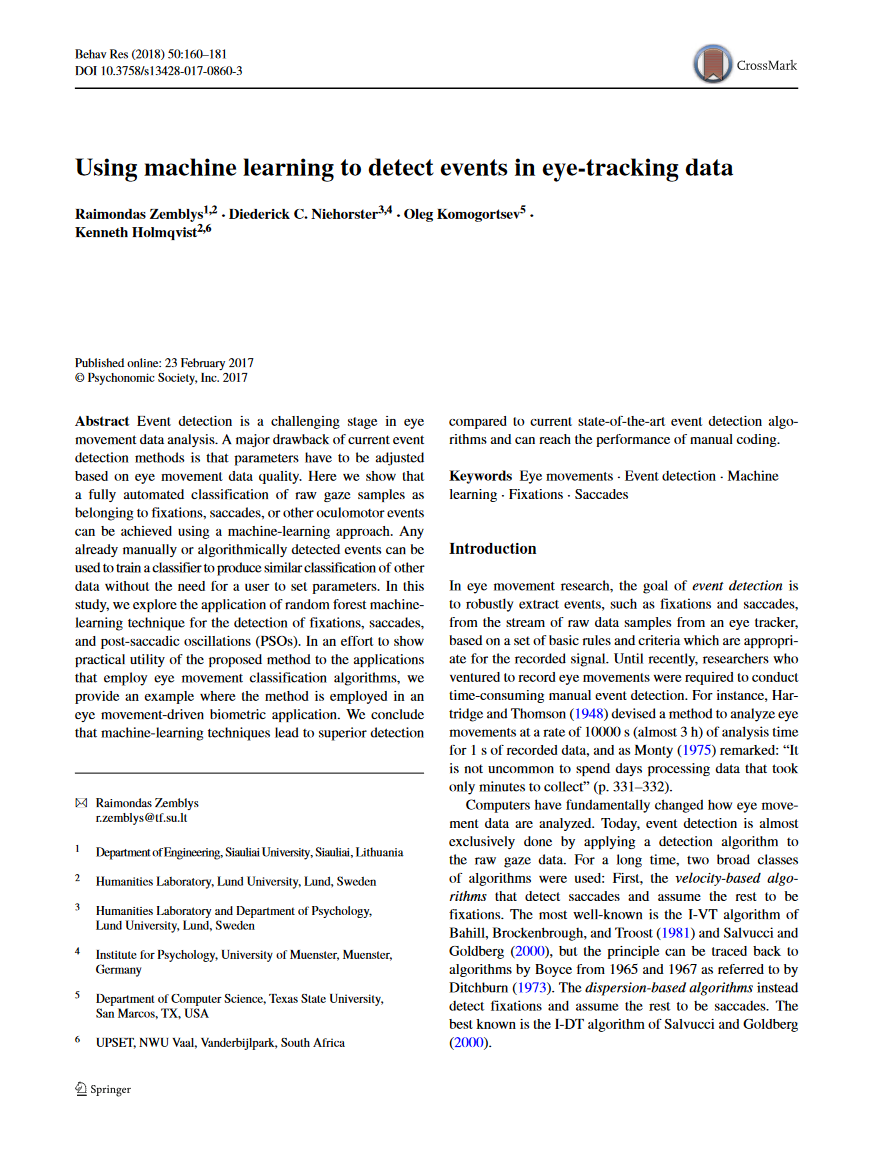
\includegraphics[width=\textwidth]{Images/DataQuality/Paper.png}
        %\caption{second figure}
    \end{minipage}
    \caption{Heat map test. Color gradient from cyan though green, then yellow to red indicate fixation duration from brief to long. The right figure shown the paper that was used to generate the heatmap.}
    \label{fig:res_PaperHeatmap}
\end{figure}

\subsection{Binary classification dataset}

Show some plot that represents the quality of labels

\subsubsection{Human error bias}

As was briefly mentioned in section \ref{sec:meth_DataLabellingEnvironments}, a bias was expected to be introduced in the dataset by human error when the user is prompted to label his own actions by mouse clicks. In figure \ref{fig:res_HumanErrorBias}, we attempt to visualise this bias by using the dispertion feature, described in further detail in section \ref{sec:meth_FeatureGeneration}. As we can see, there is very poor correlation between the peaks of xy-dispertion and each sample's labelled event. This fact reveals the major value of the post-labelling step, employed in dataset represented above. It seems that labelled saccades are lagging the dispertion peaks by a few samples, likely because the user releases the labelling button as he is moving his gaze, and simple human reaction time leads to the observed bias. Additionally, we can see that the sample period of saccade-labelled samples have little correlation with the number of samples with high values of xy-dispersion, nor the length of the saccade. This bias is likely caused by the fact that the user has no way of distinguishing the micro-differences of a 15ms saccade from a 100ms saccade, and consequently label all saccades with the same interval of button release. 

\begin{figure}[h]
    \centering
    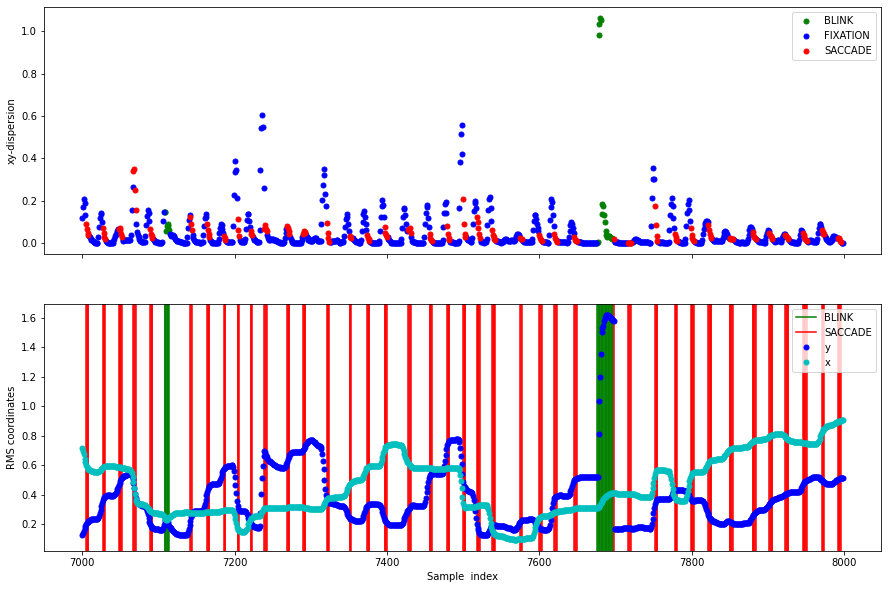
\includegraphics[width=\textwidth]{Images/Dataset/DQ_V1.png}
    \caption{Data quality from manual user labelling in static environment. The top plot show xy-dispersion and the bottom plot show x-y on-screen coordinates. Both plots are taken form a random subset of 1000 samples in the dataset. Red vertical lines and dots indicate samples where a saccade is labelled, and green vertical lines and dots indicate samples where a blink is labelled. Blue dots are samples labelled as a fixation.}
    \label{fig:res_HumanErrorBias}
\end{figure}

\subsection{Multi-class classification dataset}

Show some plot that represents the quality of labels

\subsection{Feature correlations}